\documentclass[
  jou,
  floatsintext,
  longtable,
  nolmodern,
  notxfonts,
  notimes,
  colorlinks=true,linkcolor=blue,citecolor=blue,urlcolor=blue]{apa7}

\usepackage{amsmath}
\usepackage{amssymb}




\RequirePackage{longtable}
\RequirePackage{threeparttablex}

\makeatletter
\renewcommand{\paragraph}{\@startsection{paragraph}{4}{\parindent}%
	{0\baselineskip \@plus 0.2ex \@minus 0.2ex}%
	{-.5em}%
	{\normalfont\normalsize\bfseries\typesectitle}}

\renewcommand{\subparagraph}[1]{\@startsection{subparagraph}{5}{0.5em}%
	{0\baselineskip \@plus 0.2ex \@minus 0.2ex}%
	{-\z@\relax}%
	{\normalfont\normalsize\bfseries\itshape\hspace{\parindent}{#1}\textit{\addperi}}{\relax}}
\makeatother




\usepackage{longtable, booktabs, multirow, multicol, colortbl, hhline, caption, array, float, xpatch}
\usepackage{subcaption}


\renewcommand\thesubfigure{\Alph{subfigure}}
\setcounter{topnumber}{2}
\setcounter{bottomnumber}{2}
\setcounter{totalnumber}{4}
\renewcommand{\topfraction}{0.85}
\renewcommand{\bottomfraction}{0.85}
\renewcommand{\textfraction}{0.15}
\renewcommand{\floatpagefraction}{0.7}

\usepackage{tcolorbox}
\tcbuselibrary{listings,theorems, breakable, skins}
\usepackage{fontawesome5}

\definecolor{quarto-callout-color}{HTML}{909090}
\definecolor{quarto-callout-note-color}{HTML}{0758E5}
\definecolor{quarto-callout-important-color}{HTML}{CC1914}
\definecolor{quarto-callout-warning-color}{HTML}{EB9113}
\definecolor{quarto-callout-tip-color}{HTML}{00A047}
\definecolor{quarto-callout-caution-color}{HTML}{FC5300}
\definecolor{quarto-callout-color-frame}{HTML}{ACACAC}
\definecolor{quarto-callout-note-color-frame}{HTML}{4582EC}
\definecolor{quarto-callout-important-color-frame}{HTML}{D9534F}
\definecolor{quarto-callout-warning-color-frame}{HTML}{F0AD4E}
\definecolor{quarto-callout-tip-color-frame}{HTML}{02B875}
\definecolor{quarto-callout-caution-color-frame}{HTML}{FD7E14}

%\newlength\Oldarrayrulewidth
%\newlength\Oldtabcolsep


\usepackage{hyperref}




\providecommand{\tightlist}{%
  \setlength{\itemsep}{0pt}\setlength{\parskip}{0pt}}
\usepackage{longtable,booktabs,array}
\usepackage{calc} % for calculating minipage widths
% Correct order of tables after \paragraph or \subparagraph
\usepackage{etoolbox}
\makeatletter
\patchcmd\longtable{\par}{\if@noskipsec\mbox{}\fi\par}{}{}
\makeatother
% Allow footnotes in longtable head/foot
\IfFileExists{footnotehyper.sty}{\usepackage{footnotehyper}}{\usepackage{footnote}}
\makesavenoteenv{longtable}

\usepackage{graphicx}
\makeatletter
\newsavebox\pandoc@box
\newcommand*\pandocbounded[1]{% scales image to fit in text height/width
  \sbox\pandoc@box{#1}%
  \Gscale@div\@tempa{\textheight}{\dimexpr\ht\pandoc@box+\dp\pandoc@box\relax}%
  \Gscale@div\@tempb{\linewidth}{\wd\pandoc@box}%
  \ifdim\@tempb\p@<\@tempa\p@\let\@tempa\@tempb\fi% select the smaller of both
  \ifdim\@tempa\p@<\p@\scalebox{\@tempa}{\usebox\pandoc@box}%
  \else\usebox{\pandoc@box}%
  \fi%
}
% Set default figure placement to htbp
\def\fps@figure{htbp}
\makeatother


% definitions for citeproc citations
\NewDocumentCommand\citeproctext{}{}
\NewDocumentCommand\citeproc{mm}{%
  \begingroup\def\citeproctext{#2}\cite{#1}\endgroup}
\makeatletter
 % allow citations to break across lines
 \let\@cite@ofmt\@firstofone
 % avoid brackets around text for \cite:
 \def\@biblabel#1{}
 \def\@cite#1#2{{#1\if@tempswa , #2\fi}}
\makeatother
\newlength{\cslhangindent}
\setlength{\cslhangindent}{1.5em}
\newlength{\csllabelwidth}
\setlength{\csllabelwidth}{3em}
\newenvironment{CSLReferences}[2] % #1 hanging-indent, #2 entry-spacing
 {\begin{list}{}{%
  \setlength{\itemindent}{0pt}
  \setlength{\leftmargin}{0pt}
  \setlength{\parsep}{0pt}
  % turn on hanging indent if param 1 is 1
  \ifodd #1
   \setlength{\leftmargin}{\cslhangindent}
   \setlength{\itemindent}{-1\cslhangindent}
  \fi
  % set entry spacing
  \setlength{\itemsep}{#2\baselineskip}}}
 {\end{list}}
\usepackage{calc}
\newcommand{\CSLBlock}[1]{\hfill\break\parbox[t]{\linewidth}{\strut\ignorespaces#1\strut}}
\newcommand{\CSLLeftMargin}[1]{\parbox[t]{\csllabelwidth}{\strut#1\strut}}
\newcommand{\CSLRightInline}[1]{\parbox[t]{\linewidth - \csllabelwidth}{\strut#1\strut}}
\newcommand{\CSLIndent}[1]{\hspace{\cslhangindent}#1}





\usepackage{newtx}

\defaultfontfeatures{Scale=MatchLowercase}
\defaultfontfeatures[\rmfamily]{Ligatures=TeX,Scale=1}





\title{\textbf{The MInt Scale: A Fresh Validation of the
Multidimensional Interoception Questionnaire Outperforms the MAIA, BPQ
and IAS}}


\shorttitle{MInt Validation}


\usepackage{etoolbox}









\authorsnames[{1,2},{1},{1}]{Dominique Makowski,Ana Neves,Giulia
Poreiro}







\authorsaffiliations{
{School of Psychology, University of Sussex},{Sussex Centre for
Consciousness Science, University of Sussex}}




\leftheader{Makowski, Neves and Poreiro}



\abstract{TO DO. }

\keywords{Interoception questionnaire, interoceptive accuracy scale,
MAIA, MInt Validation, Body Awareness}

\authornote{\par{\addORCIDlink{Dominique
Makowski}{0000-0001-5375-9967}}\par{\addORCIDlink{Ana
Neves}{0009-0006-0020-7599}}\par{\addORCIDlink{Giulia
Poreiro}{0000-0002-2343-5109}} 
\par{ }
\par{     \begin{tcolorbox}[enhanced jigsaw, toprule=.15mm, opacityback=0, colframe=quarto-callout-note-color-frame, left=2mm, arc=.35mm, colback=white, bottomrule=.15mm, breakable, rightrule=.15mm, leftrule=.75mm]

This preprint is a non-peer-reviewed work from the
\href{https://realitybending.github.io/}{\textbf{Reality Bending Lab}}.
\begin{center}

\includegraphics[width=0.2\linewidth,height=\textheight,keepaspectratio]{manuscript_files/mediabag/ReBeL_LogoOnly_hu114.png}
\end{center}

\end{tcolorbox}  Author roles were classified using the Contributor Role
Taxonomy (CRediT; https://credit.niso.org/) as follows:  Dominique
Makowski:   Conceptualization, Data curation, Formal Analysis, Funding
acquisition, Investigation, Methodology, Project
administration, Resources, Software, Supervision, Validation, Visualization, Writing
-- original draft; Ana Neves:   Investigation, Methodology, Project
administration, Supervision, Writing -- original draft, Writing --
review \& editing; Giulia Poreiro:   Investigation, Methodology, Writing
-- original draft, Writing -- review \& editing}
\par{Correspondence concerning this article should be addressed
to Dominique
Makowski, Email: \href{mailto:D.Makowski@sussex.ac.uk}{D.Makowski@sussex.ac.uk}}
}

\usepackage{pbalance}
% \usepackage{float}
\makeatletter
\let\oldtpt\ThreePartTable
\let\endoldtpt\endThreePartTable
\def\ThreePartTable{\@ifnextchar[\ThreePartTable@i \ThreePartTable@ii}
\def\ThreePartTable@i[#1]{\begin{figure}[!htbp]
\onecolumn
\begin{minipage}{0.485\textwidth}
\oldtpt[#1]
}
\def\ThreePartTable@ii{\begin{figure}[!htbp]
\onecolumn
\begin{minipage}{0.48\textwidth}
\oldtpt
}
\def\endThreePartTable{
\endoldtpt
\end{minipage}
\twocolumn
\end{figure}}
\makeatother


\makeatletter
\let\endoldlt\endlongtable		
\def\endlongtable{
\hline
\endoldlt}
\makeatother

\newenvironment{twocolumntable}% environment name
{% begin code
\begin{table*}[!htbp]%
\onecolumn%
}%
{%
\twocolumn%
\end{table*}%
}% end code

\urlstyle{same}



\makeatletter
\@ifpackageloaded{tcolorbox}{}{\usepackage[skins,breakable]{tcolorbox}}
\@ifpackageloaded{fontawesome5}{}{\usepackage{fontawesome5}}
\definecolor{quarto-callout-color}{HTML}{909090}
\definecolor{quarto-callout-note-color}{HTML}{0758E5}
\definecolor{quarto-callout-important-color}{HTML}{CC1914}
\definecolor{quarto-callout-warning-color}{HTML}{EB9113}
\definecolor{quarto-callout-tip-color}{HTML}{00A047}
\definecolor{quarto-callout-caution-color}{HTML}{FC5300}
\definecolor{quarto-callout-color-frame}{HTML}{acacac}
\definecolor{quarto-callout-note-color-frame}{HTML}{4582ec}
\definecolor{quarto-callout-important-color-frame}{HTML}{d9534f}
\definecolor{quarto-callout-warning-color-frame}{HTML}{f0ad4e}
\definecolor{quarto-callout-tip-color-frame}{HTML}{02b875}
\definecolor{quarto-callout-caution-color-frame}{HTML}{fd7e14}
\makeatother
\makeatletter
\@ifpackageloaded{caption}{}{\usepackage{caption}}
\AtBeginDocument{%
\ifdefined\contentsname
  \renewcommand*\contentsname{Table of contents}
\else
  \newcommand\contentsname{Table of contents}
\fi
\ifdefined\listfigurename
  \renewcommand*\listfigurename{List of Figures}
\else
  \newcommand\listfigurename{List of Figures}
\fi
\ifdefined\listtablename
  \renewcommand*\listtablename{List of Tables}
\else
  \newcommand\listtablename{List of Tables}
\fi
\ifdefined\figurename
  \renewcommand*\figurename{Figure}
\else
  \newcommand\figurename{Figure}
\fi
\ifdefined\tablename
  \renewcommand*\tablename{Table}
\else
  \newcommand\tablename{Table}
\fi
}
\@ifpackageloaded{float}{}{\usepackage{float}}
\floatstyle{ruled}
\@ifundefined{c@chapter}{\newfloat{codelisting}{h}{lop}}{\newfloat{codelisting}{h}{lop}[chapter]}
\floatname{codelisting}{Listing}
\newcommand*\listoflistings{\listof{codelisting}{List of Listings}}
\makeatother
\makeatletter
\makeatother
\makeatletter
\@ifpackageloaded{caption}{}{\usepackage{caption}}
\@ifpackageloaded{subcaption}{}{\usepackage{subcaption}}
\makeatother

% From https://tex.stackexchange.com/a/645996/211326
%%% apa7 doesn't want to add appendix section titles in the toc
%%% let's make it do it
\makeatletter
\xpatchcmd{\appendix}
  {\par}
  {\addcontentsline{toc}{section}{\@currentlabelname}\par}
  {}{}
\makeatother

%% Disable longtable counter
%% https://tex.stackexchange.com/a/248395/211326

\usepackage{etoolbox}

\makeatletter
\patchcmd{\LT@caption}
  {\bgroup}
  {\bgroup\global\LTpatch@captiontrue}
  {}{}
\patchcmd{\longtable}
  {\par}
  {\par\global\LTpatch@captionfalse}
  {}{}
\apptocmd{\endlongtable}
  {\ifLTpatch@caption\else\addtocounter{table}{-1}\fi}
  {}{}
\newif\ifLTpatch@caption
\makeatother

\begin{document}

\maketitle



\setcounter{secnumdepth}{-\maxdimen} % remove section numbering

\setlength\LTleft{0pt}




\section{Introduction}\label{introduction}

TODO: write general intro.

Main issues in existing questionnaires: - Either heavily based on
theories (e.g., focusing on a specific dimensions), despite shaky
evidence for said-theories - Do not control for context (which leads to
variability in interpretation and occurence) - Often quite narrow in the
modalities covered

\section{Study 1}\label{study-1}

TODO: write intro.

Goal of study 1: to generate a lot of items, analyze its structure and
reduce them to a balanced set of items.

\subsection{Methods}\label{methods}

\subsubsection{Participants}\label{participants}

We recruited 760 English-speaking participants using
Prolific\textcopyright. We excluded 191 for failing at least one
attention check, and 10 based on measures significantly related to the
probability of failing attention checks (namely, the multivariate
distance obtained with the OPTICS algorithm,
\citeproc{ref-theriault2024check}{Thériault et al., 2024}). The final
sample includes 559 participants (age = 37 \(\pm\) 12.2 {[}18, 77{]};
50.8\% women; Country of residence: 63.86\% United Kingdom, 26.65\%
United States). This study was approved by the University of Sussex'
Ethics Committee (\textbf{NUMBER}).

\subsubsection{Item Generation}\label{item-generation}

Based on the two goals outlined for this scale, namely to include
different interoceptive modalities, and to explicitly state the context
of the interoceptive experience (e.g., whether negative or positive), we
generated items following a combinatorial approach, where each item's
category was a combination of a specific modality and context
(Figure~\ref{fig-one}).

\begin{figure*}[!htbp]

{\caption{{The conceptual grid used to generate the 120 initial items
(top-left). Each item belong both to an interoceptive modalitiy and a
facet, with the number of each item per category indicated in the
circles. The askterisk denotes the additional presence of an attention
check item in that category. In the experiment, these items were
presented on different pages grouped either by modality (bottom-left),
by facet (top-right), or entirely randomly. The Correlation Similarity
(bottom-right) analysis suggested that the correlation matrix obtained
from the participants assigned to the random-grouping condition was
slightly more similar (but non-significantly) to the one obtained in the
modality-grouping condition, suggesting that 1) the scale's structure is
robust to different presentation conditions; 2) modality-grouping might
tend to facilitate the emergence of the underlying item structure (and
thus be interpreted as being more natural).}{\label{fig-one}}}}

\begin{center}
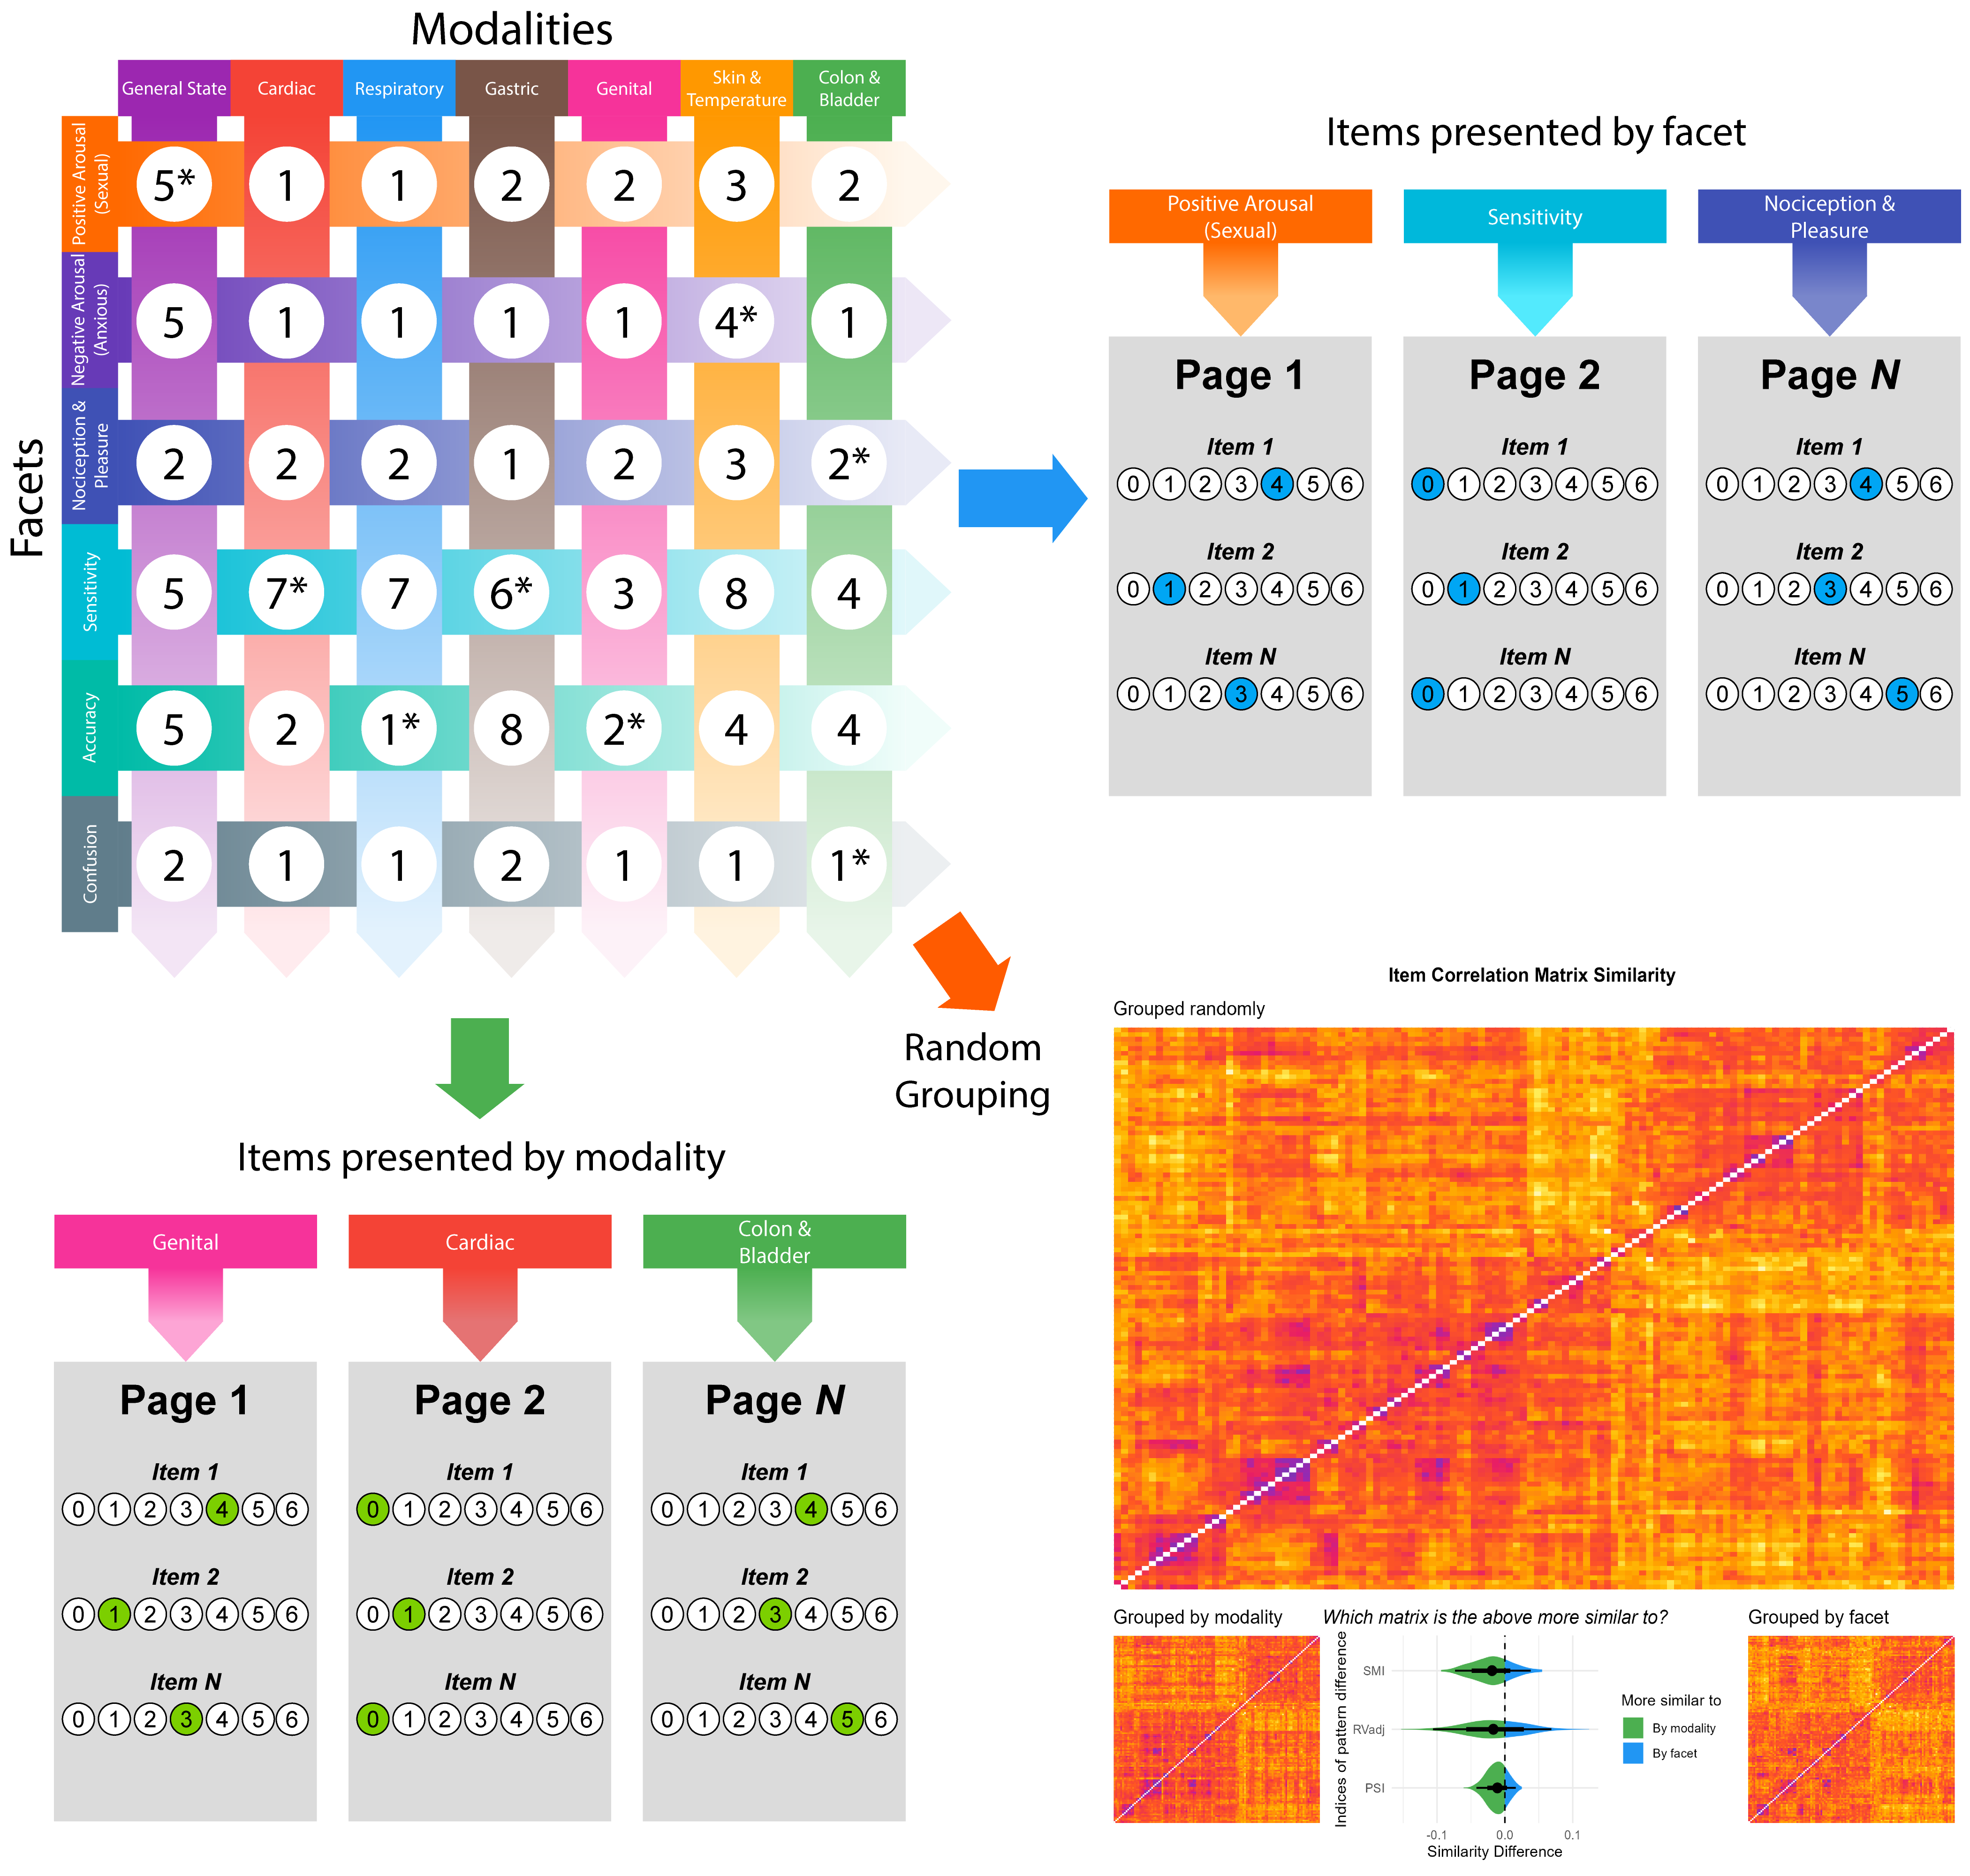
\includegraphics[width=1\linewidth,height=\textheight,keepaspectratio]{../study1/analysis/figures/figure1.png}
\end{center}

\end{figure*}

We firstly identified 7 ``modalities'' (cardiac, respiratory, gastric,
genital, skin \& temperature, bladder \& colon, and a ``general state''
category corresponding to a holistic and general awareness of an
interoceptive state or dimension). Through iterative refinement (e.g.,
splitting or merging different categories together), we then settled on
6 ``facets'', which encompass both \emph{contexts} of experience
(negative and positive arousal, namely anxious and sexual states), and
potential distinct \emph{mechanisms} (nociception \& pleasure,
sensitivity, accuracy, and confusion).

Using this orthogonal 7x6 modality/facet grid as a conceptual
scaffolding, we generated 120 initial items, striving for a balanced
number of items with consistent phrasing within modalities and
facets\footnote{The initial item list at
  \href{https://realitybending.github.io/InteroceptionScale/study1/analysis/2_analysis.html}{realitybending.github.io/InteroceptionScale/study1/analysis/2\_analysis.html}}.
We additionally crafted 8 ``attention check'' items blending in (and
distributed across) each category.

\subsubsection{Procedure}\label{procedure}

Participants were randomly assigned to one of three conditions, driving
how items were grouped on the same page: 1) items grouped by modality
(i.e., all cardiac items on the first page, all colon \& bladder items
on the second, etc.), 2) items grouped by facet, or 3) items presented
fully randomly (but balanced randomly across 6 pages). The order of the
item on any given page and the order of the modalities/facets were
randomized. Each participant completed the full set of 120 items, with
the attention check items interspersed throughout. The online experiment
was implemented using JsPsych (\citeproc{ref-de2015jspsych}{De Leeuw,
2015}), and item responses were recorded using 7-points Likert scales (0
= Disagree, 6 = Agree).

\subsubsection{Data Analysis}\label{data-analysis}

In order to test whether the grouping condition had an effect on the
structure (i.e., how items relate to one-another), we compared the
correlation matrix obtained in the random condition to the ones obtained
in the modality and facet conditions, focusing on 3 indices of
correlation matrix similarity - the Procrustes Similarity Index (PSI,
\citeproc{ref-sibson1978studies}{Sibson, 1978}), the Adjusted RV (Rvadj,
\citeproc{ref-mayer2011exploratory}{Mayer et al., 2011}), and the
Similarity of Matrices Index (SMI,
\citeproc{ref-indahl2018similarity}{Indahl et al., 2018}). For each
index, we bootstrapped the difference between the similarity with the
facet and modality conditions to test whether the correlation matrix in
the random-grouping condition is significantly more similar to any of
the two other conditions.

\subsection{Results}\label{results}

The correlation matrix similarity analysis yielded no significant
differences between the similarity of the random-grouping condition with
the modality-grouping and facet-grouping conditions
(\(PSI_{\text{Random vs. Facet}} = 0.81\),
\(PSI_{\text{Random vs. Modality}} = 0.82\), \(p = .51\);
\(RVadj_{\text{Random vs. Facet}} = 0.77\),
\(RVadj_{\text{Random vs. Modality}} = 0.78\), \(p = .78\);
\(SMI_{\text{Random vs. Facet}} = 0.49\),
\(SMI_{\text{Random vs. Modality}} = 0.51\), \(p = .55\)).

\subsection{Discussion}\label{discussion}

\section{Study 2}\label{study-2}

TODO: write intro. Goal of study 2: to validate the MInt scale against
other interoception scales.

\section{Data Availability}\label{data-availability}

Data, code, and all materials are available at
https://github.com/RealityBending/InteroceptionScale.

\section{Acknowledgements}\label{acknowledgements}

We would like to thank the dissertation students from the University of
Sussex for their help in data collection. DM would also like to thank
\ldots{} for the motivation provided to write this paper.

\section{References}\label{references}

\phantomsection\label{refs}
\begin{CSLReferences}{1}{0}
\bibitem[\citeproctext]{ref-de2015jspsych}
De Leeuw, J. R. (2015). jsPsych: A JavaScript library for creating
behavioral experiments in a web browser. \emph{Behavior Research
Methods}, \emph{47}, 1--12.

\bibitem[\citeproctext]{ref-indahl2018similarity}
Indahl, U. G., Næs, T., \& Liland, K. H. (2018). A similarity index for
comparing coupled matrices. \emph{Journal of Chemometrics},
\emph{32}(10), e3049.

\bibitem[\citeproctext]{ref-mayer2011exploratory}
Mayer, C.-D., Lorent, J., \& Horgan, G. W. (2011). Exploratory analysis
of multiple omics datasets using the adjusted RV coefficient.
\emph{Statistical Applications in Genetics \& Molecular Biology},
\emph{10}(1).

\bibitem[\citeproctext]{ref-sibson1978studies}
Sibson, R. (1978). Studies in the robustness of multidimensional
scaling: Procrustes statistics. \emph{Journal of the Royal Statistical
Society: Series B (Methodological)}, \emph{40}(2), 234--238.

\bibitem[\citeproctext]{ref-theriault2024check}
Thériault, R., Ben-Shachar, M. S., Patil, I., Lüdecke, D., Wiernik, B.
M., \& Makowski, D. (2024). Check your outliers! An introduction to
identifying statistical outliers in r with easystats. \emph{Behavior
Research Methods}, \emph{56}(4), 4162--4172.

\end{CSLReferences}






\end{document}
